\begin{frame}
\frametitle{Le travail effectu�}
\framesubtitle{Plate-forme de d�monstration (1/7)}
Architecture globale
	\begin{figure}
	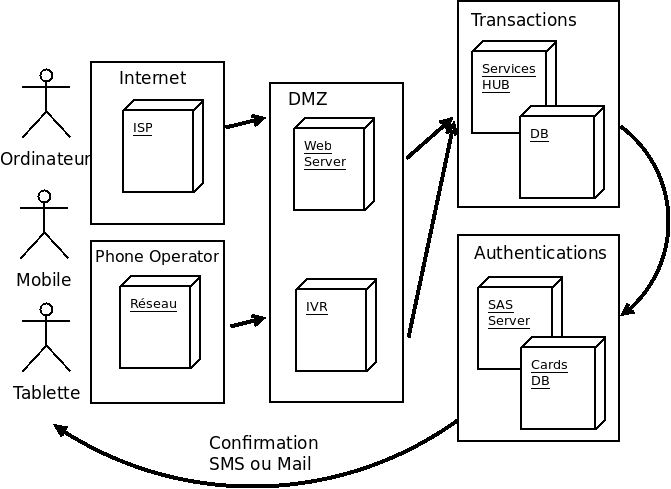
\includegraphics[scale = 0.35]{images/arch}	
	\end{figure}
\end{frame}

% ------------------------- %
\begin{frame}
\frametitle{Le travail effectu�}
\framesubtitle{Plate-forme de d�monstration (2/7)}
	\begin{block}{Deux objectifs}
	\begin{itemize}
	\item Authentification
	\item Paiement
	\end{itemize}
	\end{block}

	\begin{block}{Trois m�thode � utiliser}
	\begin{itemize}
	\item ActiveX
	\item SVI appel/rappel
	\item SVI Oneclick
	\end{itemize}
	\end{block}
\end{frame}


% ------------------------- %
\begin{frame}
\frametitle{Le travail effectu�}
\framesubtitle{Plate-forme de d�monstration (3/7)}

Principe de fonctionnement

	\begin{figure}
	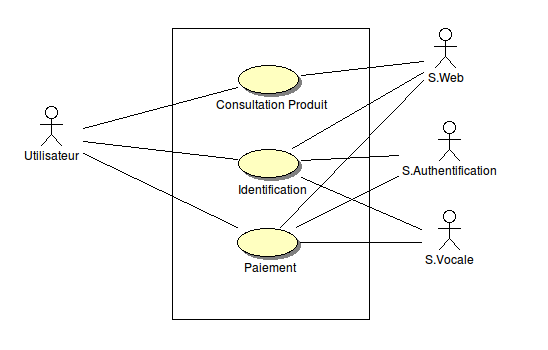
\includegraphics[scale = 0.5]{images/uml1}	
	\end{figure}
\end{frame}

% ------------------------- %
\begin{frame}
\frametitle{Le travail effectu�}
\framesubtitle{Plate-forme de d�monstration (4/7)}

	\begin{figure}
	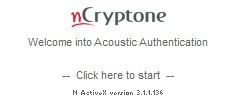
\includegraphics[scale = 0.7]{images/ax}	
	\end{figure}
\begin{center}
L'utilisateur doit cliquer dans l'ActiveX pour initialiser la capture acoustique.
\end{center}
	\begin{block}{ActiveX}
	\begin{itemize}
	\item HTTP
	\item JAVASCRIPT
	\end{itemize}
	\end{block}
\end{frame}
% ------------------------- %
\begin{frame}
\frametitle{Le travail effectu�}
\framesubtitle{Plate-forme de d�monstration (5/7)}

Fonctionnement serveur vocal (SVI)
	\begin{figure}
	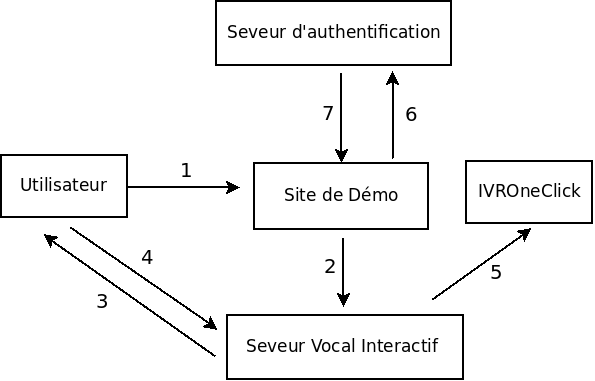
\includegraphics[scale = 0.4]{images/Diagramme1}	
	\end{figure}
\end{frame}


% ------------------------- %
\begin{frame}
\frametitle{Le travail effectu�}
\framesubtitle{Plate-forme de d�monstration (6/7)}

	\begin{block}{SVI}
Le dialogue entre le SVI et le serveur web se fait � l'aide de 2 pages Web
	\begin{itemize}
	\item GET\_Session
	\item POST\_RAW
	\end{itemize}
	\end{block}

	\begin{block}{Les param�tres}
	\begin{itemize}
\begin{columns}
\begin{column}[l]{0.4\textwidth}
	\item PhoneNumberToCall 
	\item DemoID
	\item InternalPINCardRange1
\end{column}
\begin{column}[r]{0.4\textwidth}
	\item InternalPINCardRange2
	\item SessionID
	\item AskPIN
\end{column}
\end{columns}
	\end{itemize}
	\end{block}

\end{frame}





% ------------------------- %
\begin{frame}
\frametitle{Le travail effectu�}
\framesubtitle{Plate-forme de d�monstration (7/7)}
\centering
\textbf{D�monstration}

	\begin{figure}
	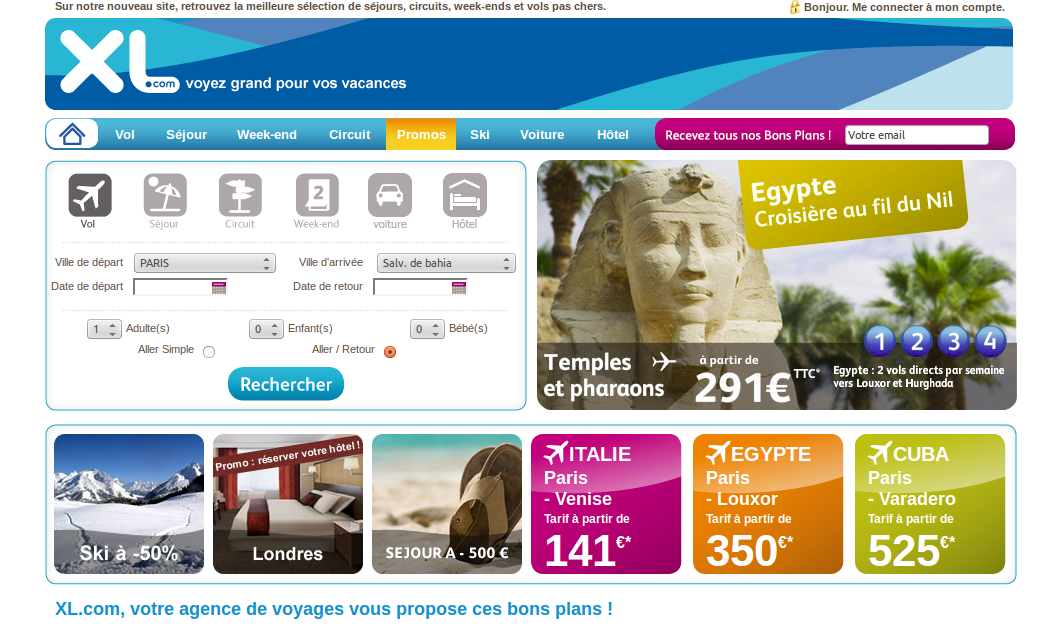
\includegraphics[scale = 0.2]{images/d3}	
	\caption{\url{http://solution.uint.fr/xlplus/}}
	\end{figure}
\end{frame}
